\section{Coupling experiment}
After a pilot study \cite{Harmon2016b}
we conducted an experiment to study how 
coupling digital and physical models of topography 
mediates 3D spatial performance. 
%
This experiment compared how users performed 
in a terrain modeling task using 
digital 3D modeling with Rhinoceros, 
analog modeling by hand, 
and projection-augmented modeling powered by Tangible Landscape. 
% digital
Digital modeling with a GUI affords precise transformations and
dynamic modes of visualization such as 
3D orbiting, zooming, and ray traced shading,
but is not embodied.
% analog
Theoretically analog modeling -- modeling by hand or with tools -- 
should be embodied, 
affording subconscious, kinaesthetic sensing and manipulation of form. 
By sensing form subconsciously with the body
users should have more cognitive resources for critiquing their work 
and strategizing their next moves. 
% 
Projection-augmented modeling 
couples digital mapping with physical modeling.
Theoretically it should combine affordances of both -- 
enabling enriched visualization and physical sensing and manipulation -- 
to offer more feedback.
While more feedback may help users 
better assess and critique their performance 
so they can strategize their next moves,
too much feedback may be a cognitive overload 
resulting in distraction, frustration, and demotivation. 
Physical sensing and manipulation, however, should offload 
some of this cognitive work onto the body.

\subsection{Methods}
In this experiment 
18 participants tried to accurately model a given study landscape 
digitally, by hand, and with Tangible Landscape. 

\paragraph{Participants}
All of the participants 
-- either graduate students, faculty, or professionals 
in landscape architecture or geographic information science -- 
had experience thinking spatially. 
These participants were selected in order to compare 
the performance of novices and experts
in grading (i.e.~earthworking), GIS, and 3D modeling.
Of the 12 graduate students 6 were in the \nth{2} semester of the 
Master of Landscape Architecture program 
at North Carolina State University.
These students were just beginning to learn to read and manipulate contour lines 
in the class Landform, Site Grading, and Development Systems. 
They had no experience with GIS, 3 credit hours of training in digital representation, 
and no experience with Rhinoceros.
The other 6 graduate students were in the \nth{2} semester of the 
Master of Geospatial Information Science and Technology program 
at North Carolina State University.
They had at least 9 credits hours of training in GIS, but 
had no experience with contour maps, digital terrain modeling, or 3D modeling.
The other 6 participants were either landscape architecture faculty 
with professional experience or practicing professionals in landscape architecture 
from around the world. 
Of these 2 were experts in 3D modeling with over 10 years of experience 
using Rhinoceros and similar programs including Maya and 3ds Max. 
These experts felt comfortable and proficient modeling a wide variety of geometries 
and had developed unique, personalized, and highly adaptable workflows 
(see Table~\ref{table:participants}).

\begin{table}
\tbl{Participants}{
\ra{1.3}
\begin{tabular}{l <{\hspace{1em}} c <{\hspace{1em}} c <{\hspace{1em}} c}
\toprule
Group & No. & GIS training & 3D modeling expertise \\
\midrule
Landscape architecture students & 6 & 0 & 0\\
GIS students & 6 & 6 & 0\\
Academics \& professionals & 6 & 0 & 2\\
\bottomrule
\end{tabular}}
\label{table:participants} 
\end{table}

\paragraph{Experimental design}
% tasks
Participants were given three tasks -- 
to digitally sculpt a model of a landscape using the 3D modeling program Rhinoceros, 
to hand sculpt a model of a landscape in polymer-enriched sand,
and to sculpt a model of a landscape using Tangible Landscape.
% time limit 
They had 10 minutes to complete each task. 
The time limit was calibrated based on 
the time it took the research team 
to comfortably complete each task. 
% counterbalancing / order of tasks
The modeling tasks were reordered for each participant
to partially account for learning and fatigue
by counterbalancing the experiment using a Latin square design.
% assessment
Participants were asked to model the same landscape for each task 
so that their performance could be quantitatively assessed 
using spatial modeling, statistics, analysis, and simulation.
Their modeling processes were qualitatively assessed 
through direct observation
supported by photographic and video documentation. 
% 
After completing the tasks
the academics and professionals 
were interviewed. 
We intended to conduct semi-structured interviews 
with all of the participants, but
the students were too tired by the end of the experiment. 
%
Psychometric tests were not used
to assess spatial ability because
these do not address 
geographic scales,
spatial relations,
domain-specific knowledge and abilities 
\cite{Lee2009,Bednarz2011,Wakabayashi2011},
or embodied cognitive ability. 
%
See Appendix 
\ref{appendix:procedure} for instructions for running the experiment
and Appendix 
\ref{appendix:guidelines} for semi-structured interview guidelines. 

% study landscape
We used a region of Lake Raleigh Woods in Raleigh, North Carolina 
as the study landscape for this experiment. 
A real landscape was used because computer generated landscapes 
often look surreal and may lack distinct landforms and clearly defined streams. 
This study region has distinctive, 
clearly defined landforms -- a stream valley flanked by a ridge and sloping towards the lake.
%(see Table~\ref{table:coupling_experiment}). 
The digital elevation model for this region was derived from a 2013 airborne lidar survey 
using the regularized spline with tension interpolation method \cite{Mitasova2005}. 
% physical reference models
We CNC routed a model of the study landscape in Baltic birch 
using 2 parallel finish cuts 
with a 3.175 mm diameter ball-nose bit
with a 1.27 mm stepover. 
Participants were given this model 
at the beginning of the experiment
to use as a reference during each task.

%\begin{figure}
%\begin{center}
%	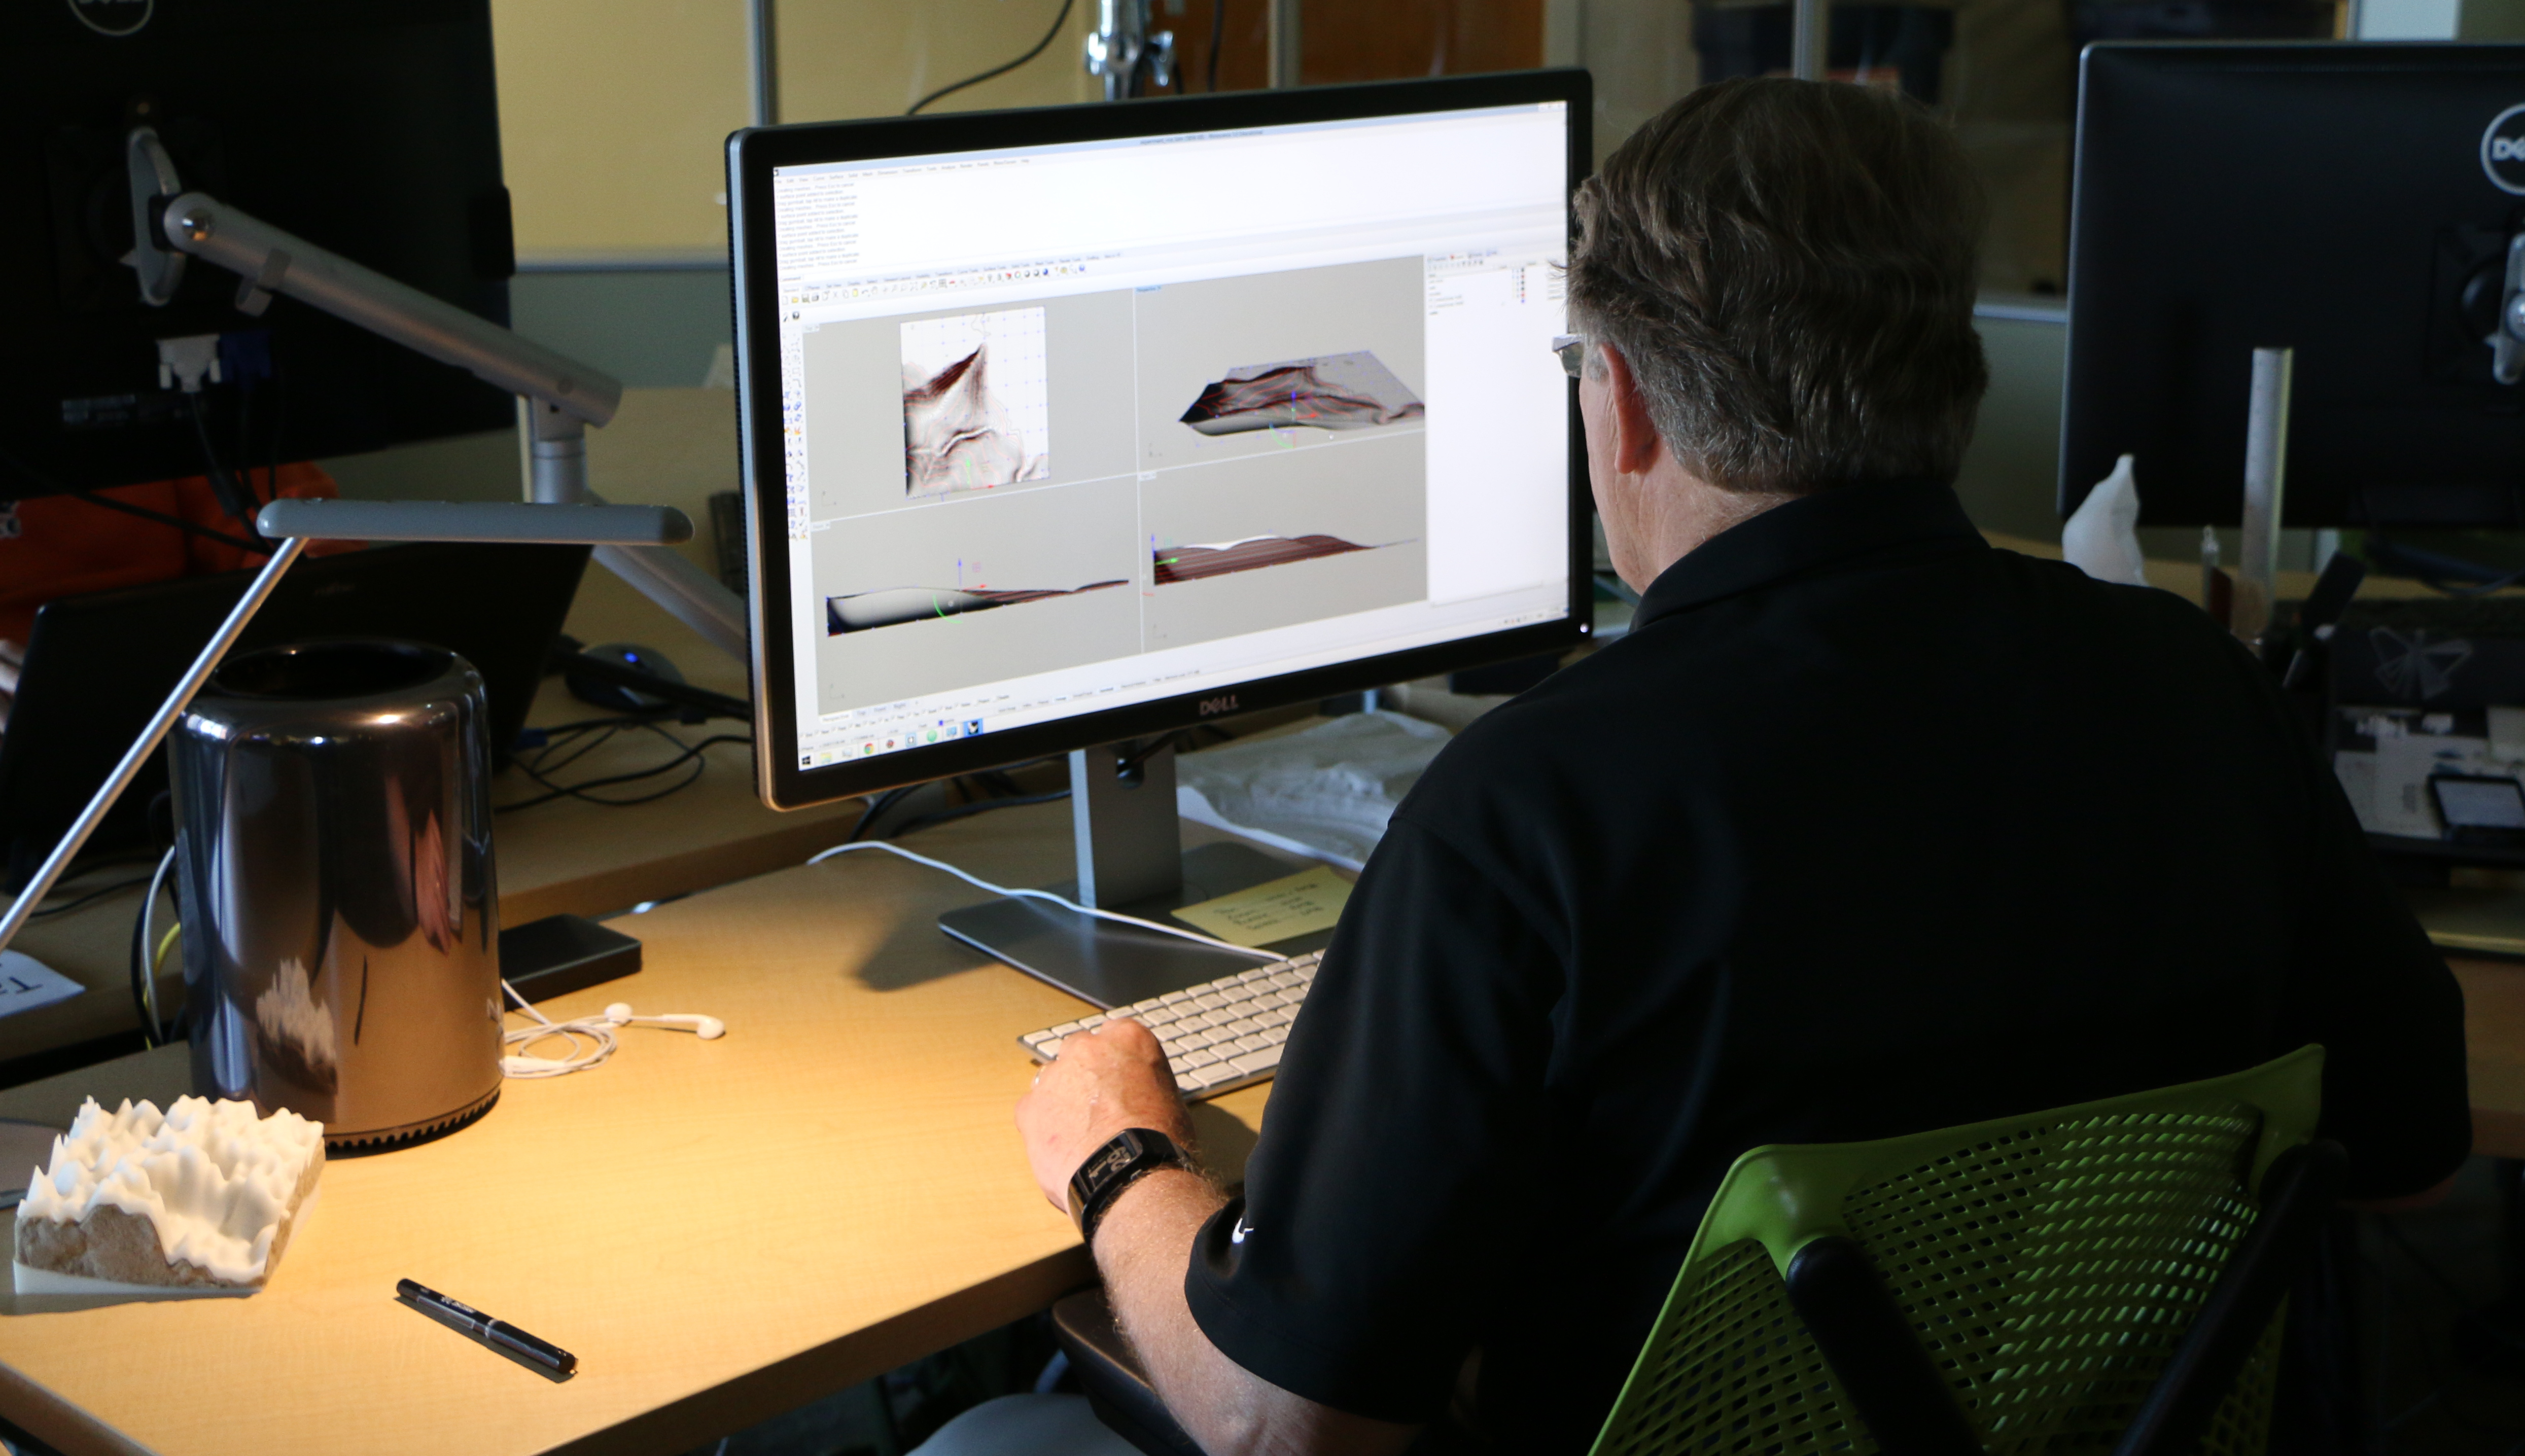
\includegraphics[height=108px]{images/experiments/art_rhino.jpg}
%	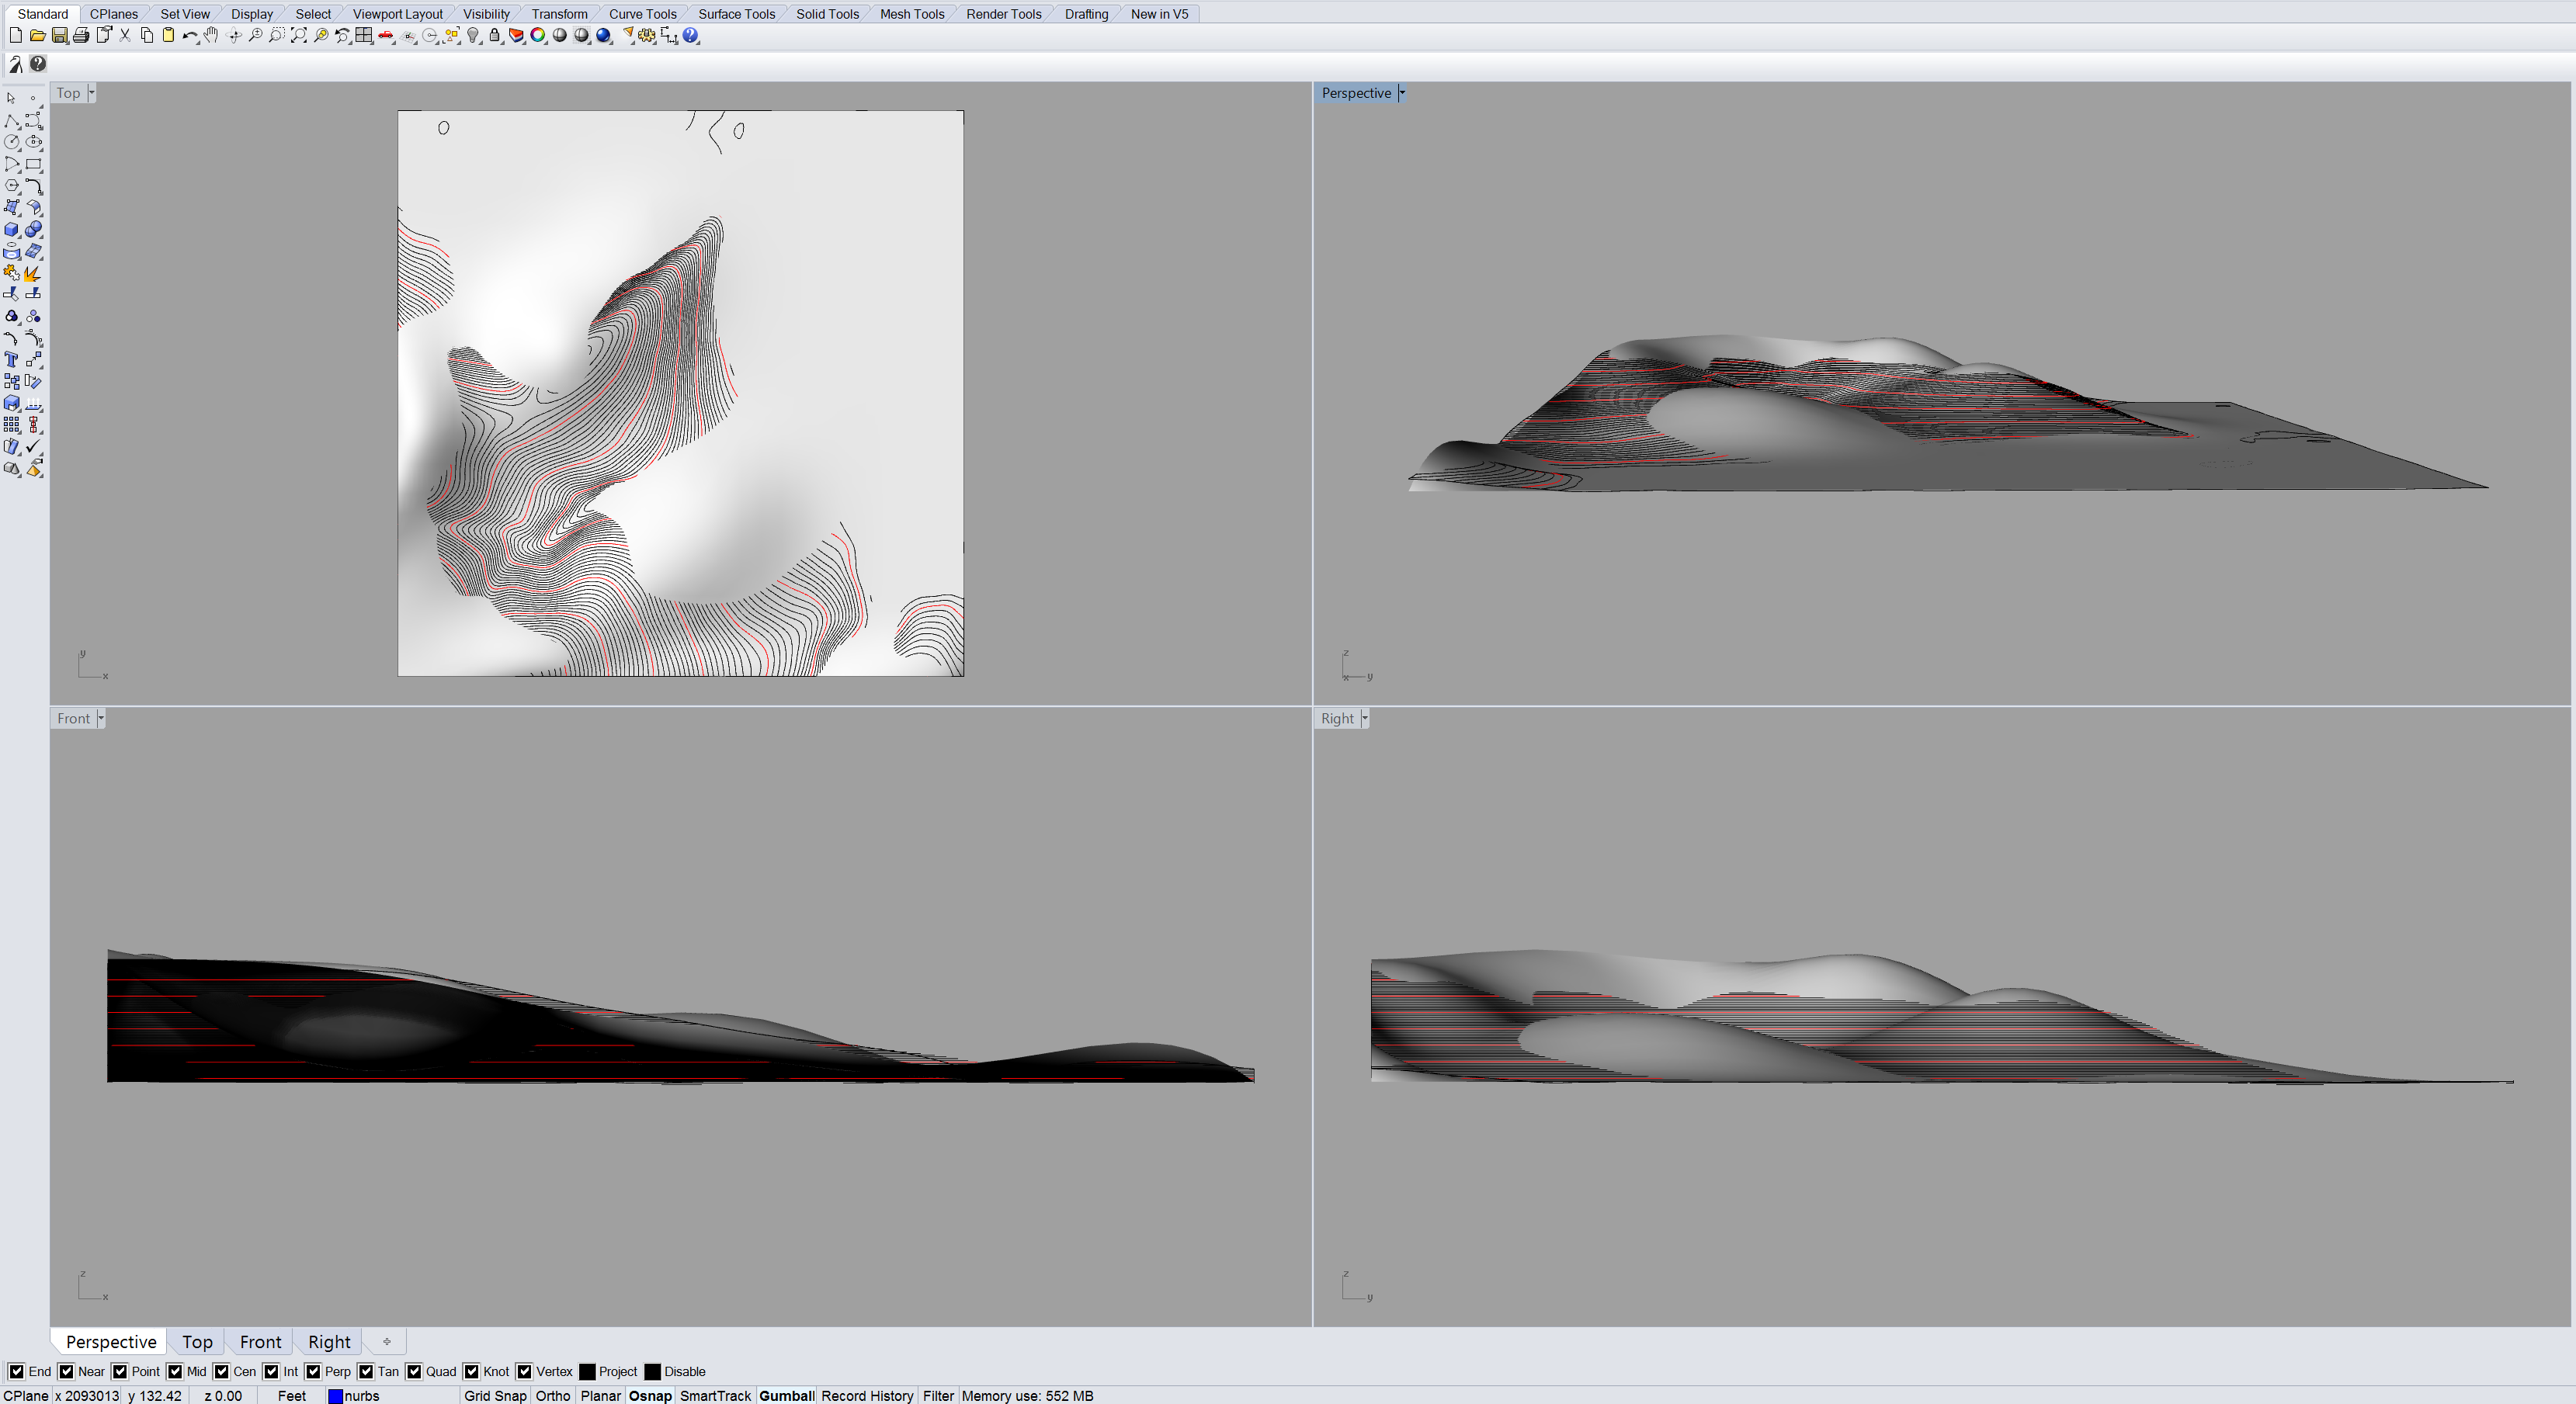
\includegraphics[height=108px]{images/experiments/rhino.png}
%	\caption{Coupling experiment -- digital modeling.
%	A participant digitally sculpts the study landscape in Rhinoceros
%	using 3D contours as guides.}
%	\label{fig:rhino}
%	%
%	\vspace*{0.5em}
%	%
%	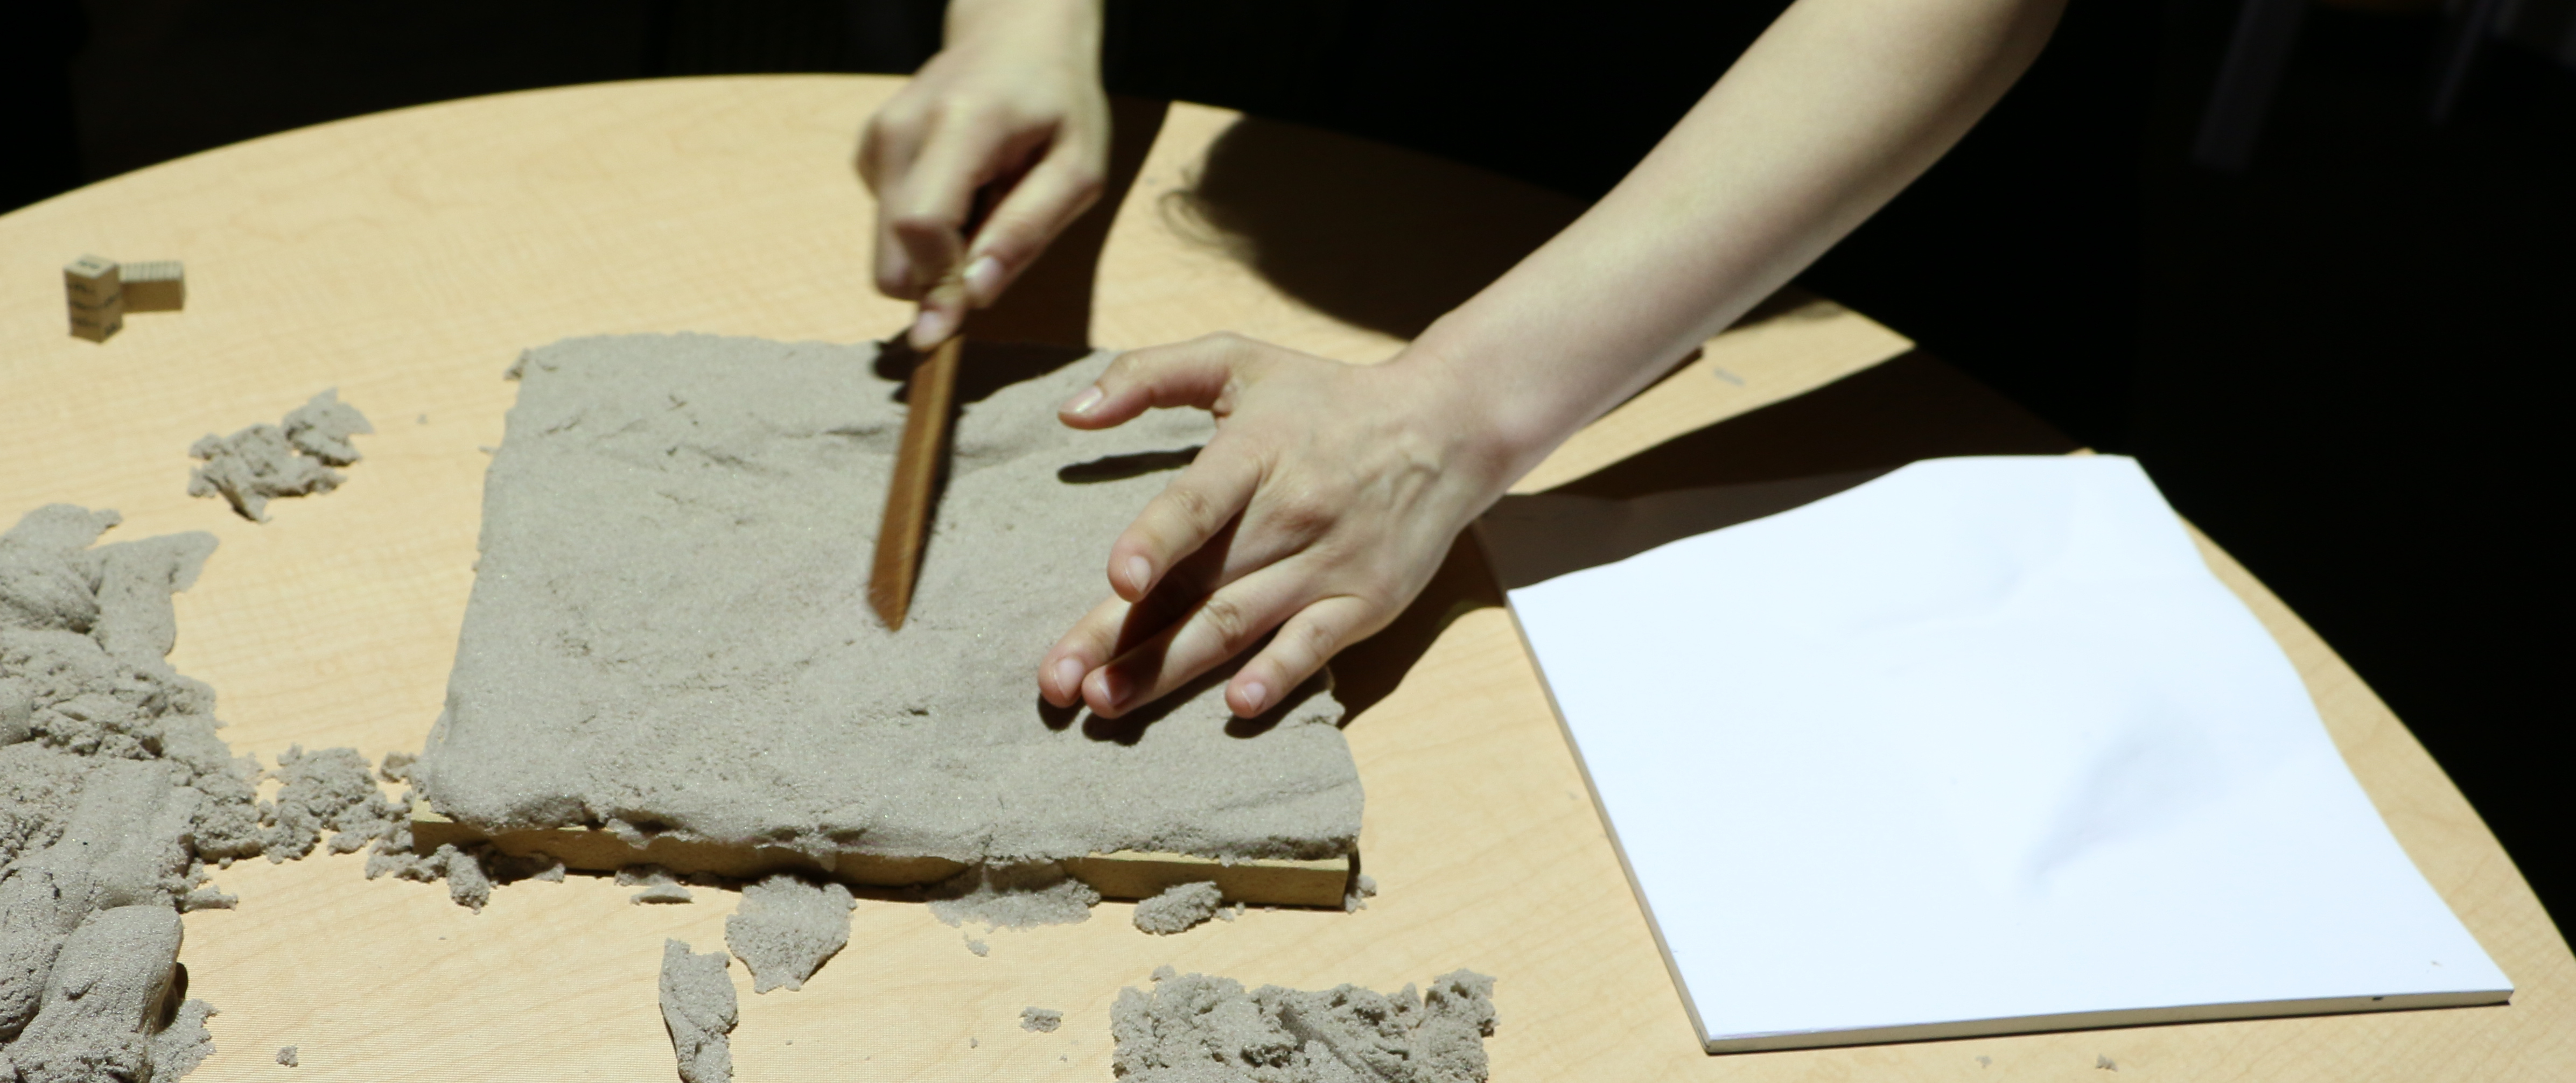
\includegraphics[width=\textwidth]{images/experiments/connie_analog_1.jpg}
%	\caption{Coupling experiment -- analog modeling by hand.
%	A participant sculpts the study landscape by hand
%	using a physical model as a reference.}
%	\label{fig:analog}
%	%
%	\vspace*{0.5em}
%	%
%	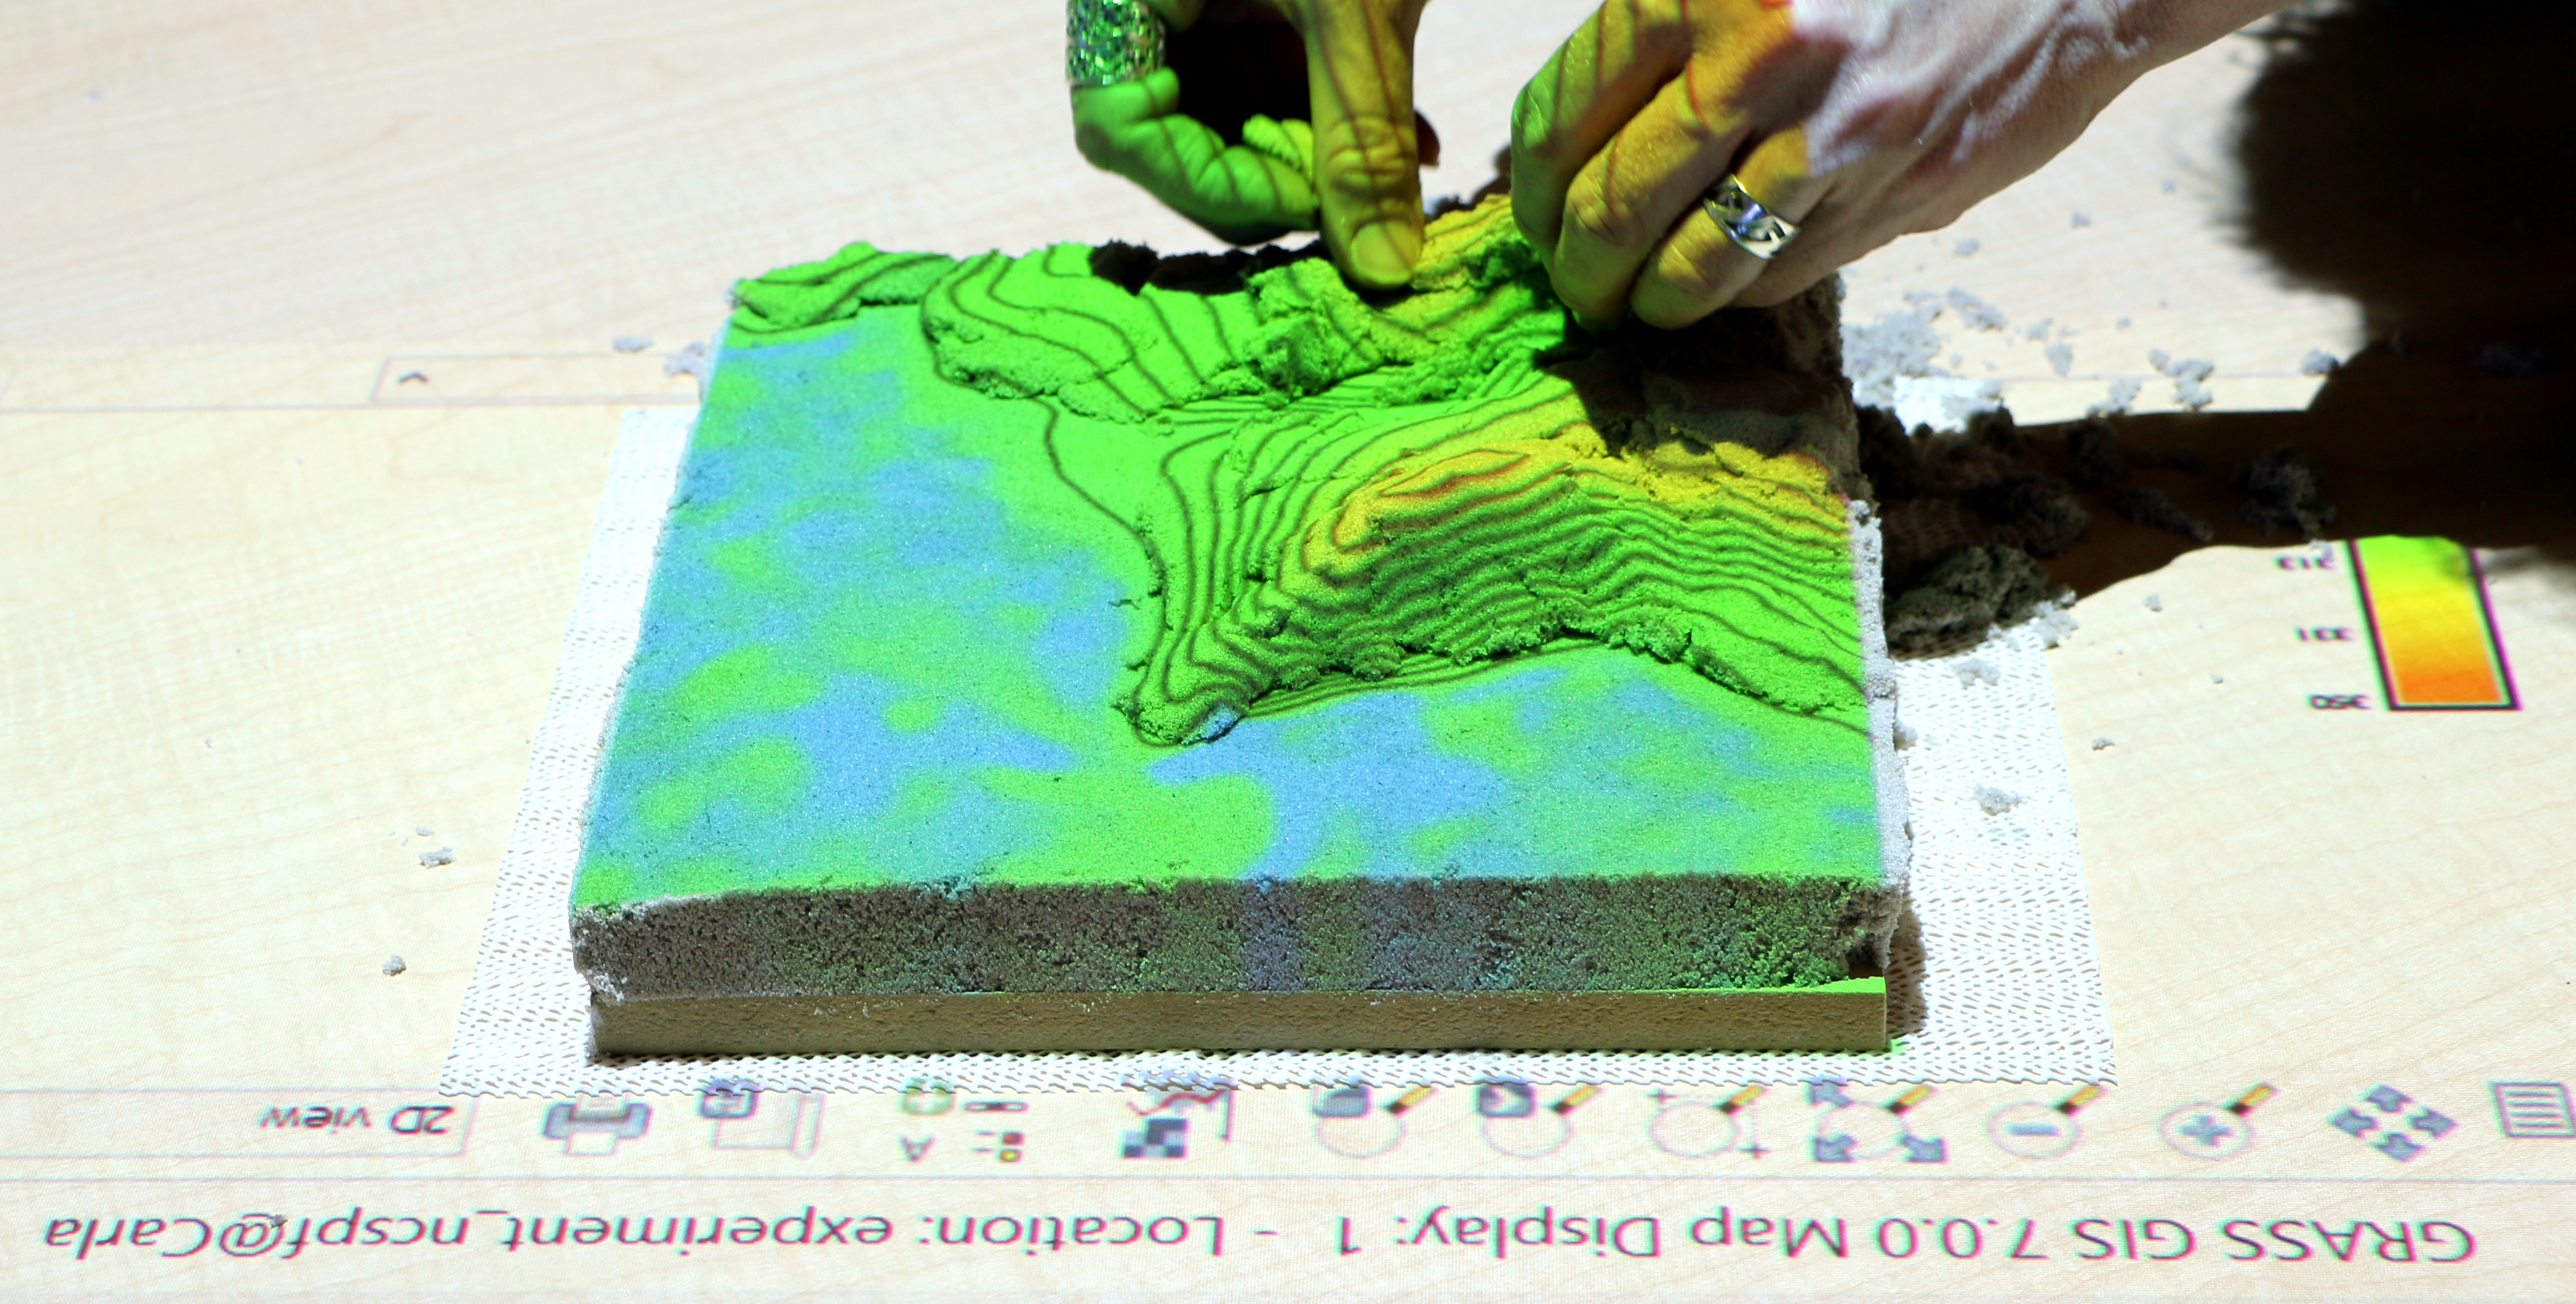
\includegraphics[width=\textwidth]{images/experiments/carla_proj_aug.jpg}
%	\caption{Coupling experiment -- projection-augmented modeling.
%	A participant sculpts the study landscape using
%	the projected elevation and contour maps
%	as guides.}
%	\label{fig:proj_aug}
%\end{center}
%\end{figure}


\paragraph{Digital modeling}
Participants had 10 minutes 
to digitally model the study landscape in Rhinoceros 5, 
a non-uniform rational basis spline 
(NURBS) based 3D modeling program
designed for precise freeform curve and surface modeling \cite{Rhino}.
After 10 minutes of training 
participants modeled the study landscape as a NURBS surface 
by vertically translating control points (Fig.~\ref{fig:rhino}). 
They started with a flat NURBS surface that was 
divided into a 10 x 10 grid of control points.
As a reference their model space also included 
a locked representation of the study landscape as 3D contours. 
At any point participants could rebuild the surface 
with a higher density of control points for finer, more nuanced control. 
This method is relatively simple and 
analogous to basic actions in sculpture -- pushing and pulling. 
We developed and tested this method 
as a simple, straightforward technique for  
digital freeform surface modeling
that could be taught quickly, yet could produce an accurate model. 
%  
% timing / rebuilding
Through testing we determined that 
novice users took approximately 10 minutes
to model the surface with a 10 x 10 grid of control points
before wanting to rebuild the surface with more control points.
%
See Appendix \ref{appendix:experiment_videos}
for videos demonstrating the training (\ref{videos:training}) 
and digital 3D modeling task (\ref{videos:digital}).

% choice of 3d modeling program
Different 3D modeling programs afford very different
interactions, modeling tools, data structures, and modes of representations. 
%
Developing a simple, intuitive modeling technique 
drove the choice of software in this study. 
%
After testing 3D modeling workflows in 
Rhinoceros, Vue, Maya, and SketchUp
we chose Rhinoceros 5 for this task because it 
is popular with designers such as architects, 
has a wide variety of modeling tools,
can precisely represent continuous surfaces, 
and has plugins for importing and exporting geographic data. 
%
To make a fair comparison 
between digital, analog, and tangible modeling,
the digital modeling technique 
needed to be relatively analogous to hand sculpting
-- i.e.~pushing and pulling rather than painting in 3D, 
drafting in 3D, or stacking voxels.
%
There is an analogous modeling technique 
-- pulling and pushing vertices -- 
using the Sandbox tool in SketchUp \cite{SketchUp},
but this creates a triangulated irregular network (TIN)
rather than a continuous NURBS surface. 
%
Vue has a terrain editor designed for intuitive 3D painting and sculpting \cite{Vue},
but it requires continual retuning of tool parameters
and generates a TIN. 
%
TINs less accurately represent continuous surfaces like topography
and would generate artifacts in our analyses. 
%
In another pilot study \cite{Harmon2016} 
we tested Vue's terrain editor. 
We found that participants tended to 
over-exaggerate distinct features 
in the landscape like stream channels, 
while ignoring more subtle features like slopes.  
We also determined that the resulting models
had an obvious triangulated structure that caused
exaggerated slopes and discontinuous water flow 
in our analyses. 
%
While voxel modeling programs 
like Voxel Builder % http://voxelbuilder.com/
%and MagicaVoxel % https://ephtracy.github.io/
and games like Minecraft \cite{Minecraft}
are very intuitive to use,
they can also be slow to use,
create blocky rather than
continuous surfaces, 
and are not typically used in design professions 
like architecture and landscape architecture.

\paragraph{Analog modeling}

After a brief explanation and demonstration
participants had 10 minutes to sculpt 
the study landscape in polymer-enriched sand 
by hand or with a wooden sculpting tool (Fig.~\ref{fig:analog}).  
They were given a CNC-routed model of the study landscape 
as a reference, a sculpting tool, and a 3D scale. 
Participants were shown how the 3D scale could be used to 
measure the height of the model. 
A lamp on the table cast shadows across the model for hillshading.
%
See Appendix \ref{appendix:experiment_videos}
for a video demonstrating the analog 3D modeling task (\ref{videos:analog}).

\paragraph{Projection-augmented modeling}
After a minute long explanation and demonstration
participants had 10 minutes to sculpt
a projection-augmented, polymer-enriched sand model
of the study landscape by hand or with a wooden sculpting tool 
(Fig.~\ref{fig:proj_aug}). 
Tangible Landscape was used to project 
an elevation map of the study landscape
with contours and a legend
onto participants' sand models as guide for sculpting. 
Participants were also given CNC routed reference model and 
a 3D scale ruled in map units. 
After an explanation of the contour map, elevation color table, and legend,
participants were shown how the 3D scale could be used to 
measure the elevation of their scale models.
%
See Appendix \ref{appendix:experiment_videos}
for a video demonstrating the projection-augmented 3D modeling task (\ref{videos:augmented}).

\paragraph{Data collection and analysis}
We used Tangible Landscape to scan the finished models 
built using analog hand modeling and projection-augmented modeling.
The scans were captured as point clouds, interpolated 
as digital elevation models 
using the regularized spline with tension method,
and stored as raster maps in a GRASS GIS database. 
The NURBS surfaces modeled in Rhinoceros 
were exported as raster elevation maps,
imported into GRASS GIS, randomly resampled, 
re-interpolated using the regularized spline with tension method, 
and stored as raster maps in a GRASS GIS database. 
The data from Rhinoceros 
was randomly resampled and re-interpolated to account for 
differences and irregularities in resolution, data density, and point spacing.
%
For each set of models -- digital, analog, and augmented --
we computed raster statistics (i.e.~per cell statistics), 
topographic and morphometric parameters, 
and simulated water flow.

\paragraph{Mean elevation}
We computed 
the mean elevation 
and standard deviation of elevation
for each set
with the module \textit{r.series} \cite{r.series}.
The mean elevation is the average of each cell 
of all elevation maps in a given set of models.

\paragraph{Standard deviation of elevation}
The standard deviation of elevations 
represents the set's consistency.
We computed 
the standard deviation of elevation for each set
with the module \textit{r.series} \cite{r.series}.
This is the standard deviation of each cell 
of all elevation maps in a given set of models.
We used a sequential color table from Color Brewer
\cite{Brewer1994,ColorBrewer}.

\paragraph{Mean difference}
In order to compare participants' modeling performance 
between sets we computed the difference 
between the linearly regressed reference elevation and 
the mean elevation for each set.
%
The difference between the reference 
and mean elevation maps should show
where the mean elevation values for each set 
are too low or too high, 
i.e.~where they needed to add (blue) 
or remove (red) volume to match the reference. 
%
There were, however, systematic errors 
in the scanned models.
%
Table \ref{table:scatterplots} shows the vertical shift 
in the hand sculpted and projection-augmented models 
caused by scanning and georeferencing.
%
We used linear regression 
to vertically rescale and translate the reference elevation 
in order to account for these systematic errors
in the difference calculation,

\begin{equation}
\label{eq:regressed_mean_difference}
\Delta = (a + b * z_0) - \overline{z}
\end{equation}

where:

\hspace*{1em} $\Delta$ is the difference

\hspace*{1em} $z_0$ is the reference elevation map

\hspace*{1em} $\overline{z}$ is the mean elevation of maps in a set

\hspace*{1em} $a$ is the intercept of the regression line

\hspace*{1em} $b$ is the slope of the regression line.\\


\paragraph{Standard deviation of difference}
In order to find 
how consistently the models fit the reference landscape
we computed the standard deviation of difference
by first calculating the difference 
between the linearly regressed reference elevation and 
each modeled elevation map in a set
to generate a set of difference maps.
Then we calculated the standard deviation 
for that set of difference maps.  



\paragraph{Mean slope}
We derived the slope of the mean elevation of each set 
using differential geometry
\cite{Wood1996} 
with the module \textit{r.param.scale} \cite{r.param.scale}.

\paragraph{Mean landforms}
We identified landforms 
for the mean digital elevation model for each set 
using geomorphons,
a pattern recognition method for landform classification 
based on the openness of the terrain
and implemented as the add-on module \textit{r.geomorphon} \cite{r.geomorphon}.
Geomorphon works effectively across spatial scales because 
the neighborhood search size for pattern recognition 
is spatially variable -- it depends on the visibility of the cell \cite{Jasiewicz2013}.  
Landforms can be classified as flat, peak, ridge, shoulder, spur, slope, hollow, footslope, valley, or depression (Fig.~\ref{fig:geomorphons}).

\paragraph{Mean minimum distance}
We computed the mean minimum distance between cells
with water flow, ridges, and valleys
on the models and the reference landscape
as a measure of positional accuracy. 

\paragraph{Systematic errors}
Table \ref{table:scatterplots} shows systematic errors
in the hand sculpted and projection-augmented models.
These models are vertically shifted due to scanning
and have low values along the borders
caused by slumping sand. 
While we used linear regression 
to vertically shift and rescale the difference in elevation, 
we did not mitigate the systematic errors
along the borders. 
